\documentclass[10pt,twocolumn]{article}

\usepackage[left=0.62in,right=0.62in,top=0.62in,bottom=0.68in]{geometry}
\usepackage{amsmath,amssymb,mathtools}
\usepackage{booktabs}
\usepackage{graphicx}
\usepackage{float}
\usepackage[hidelinks]{hyperref}
\usepackage{microtype}

\setlength{\columnsep}{0.25in}
\setlength{\parindent}{1em}
\setlength{\parskip}{0pt}
\allowdisplaybreaks

\newcommand{\ii}{\mathrm i}
\newcommand{\R}{\mathbb R}
\newcommand{\C}{\mathbb C}
\newcommand{\I}{I}
\newcommand{\Tr}{\operatorname{Tr}}
\newcommand{\norm}[1]{\lVert#1\rVert}
\newcommand{\MB}{M_{\mathrm B}}

\title{Compact Divergence and Representability Analysis of the Archive
Electron--Phonon Equations of Motion}
\author{Jake Strobel}
\date{August 2026}

\begin{document}
\maketitle

\begin{abstract}
For the two-site Holstein dimer, the matrix electron--phonon moment equations
are reduced by a block-affine coordinate decomposition to 31 independent real
variables.  Positivity of the electronic density and joint electron--phonon
Gram matrices defines the tested positive-semidefinite cone, supplemented by
fixed-particle-number trace conditions.  The uncorrected trajectory leaves
this physical domain before its later coordinate blow-up.  At every
Runge--Kutta stage, a minimum-Euclidean-norm correction is added to the
velocity subject to differential positivity barriers, the trace conditions,
and zero instantaneous correction-induced internal-energy flux.  This
correction prevents divergence and preserves representability through
$t=1000\,t_{\rm hop}^{-1}$, although comparison with exact
truncated-Hamiltonian propagation shows that strong-coupling observable errors
remain substantial.  Extending the hierarchy through all symmetry-adapted
moments of total degrees three and four makes the lower-order derivatives
nearly exact but transfers the dominant defect to the newly highest retained
order.  The correction therefore resolves the loss of representability
without resolving the moment-closure error; current work seeks a physically
adapted closure that also improves observable accuracy.
\end{abstract}

\section{Archive moment equations and block-affine reduction}

The calculation uses the two-site, two-electron Holstein Hamiltonian in the
one-spin-up/one-spin-down sector, with $t_{\rm hop}=1$,
$\omega_{\rm ph}=0.5$, $g=\sqrt{3/8}$, and
$V(t)=2\sin(\pi t/4)e^{-t^2/2}$.  Exact diagonalization with local phonon
occupations $0\leq n_q^{\rm ph}\leq16$ supplies the initial ground-state
contractions.  Suppressing the spin-up label on the one-body electronic
operators, define
\begin{equation}
\begin{gathered}
\rho_{ij}=\langle c_j^\dagger c_i\rangle,
\qquad B_q=\langle b_q\rangle,
\qquad \delta b_q=b_q-B_q,\\
N_{qr}=\langle\delta b_r^\dagger\delta b_q\rangle,
\qquad A_{qr}=\langle\delta b_q\delta b_r\rangle,\\
C^q_{ij}=\langle\delta b_q(c_j^\dagger c_i-\rho_{ij})\rangle,
\qquad X=(\rho,B,N,A,C^0,C^1).
\end{gathered}
\label{eq:moments}
\end{equation}
Here $i,j,q,r\in\{0,1\}$ label electronic sites or phonon modes as
appropriate.  For $G_q=g|q\rangle\langle q|$, spin multiplicity $\nu=2$,
and $\omega_0=\omega_1=\omega_{\rm ph}$, define
\begin{equation}
h(t)=
\begin{pmatrix}V(t)/2&-t_{\rm hop}\\-t_{\rm hop}&-V(t)/2\end{pmatrix}
+\sum_{q=0}^{1}G_q(B_q+B_q^*).
\label{eq:one-body-h}
\end{equation}
The archive matrix equations specialize to
\begin{subequations}\label{eq:dimer-eoms}
\begin{align}
\Phi_{ij}&=-\ii g[C^i_{ij}+(C^i_{ji})^*],\\
\dot\rho&=-\ii[h(t),\rho]+\Phi+\Phi^\dagger,\\
\dot B_q&=-\ii(\omega_qB_q+\nu g\rho_{qq}),\\
\dot N_{qq'}&=-\ii(\omega_q-\omega_{q'})N_{qq'}\\
&\quad+\ii\nu gC^q_{q'q'}-\ii\nu g(C^{q'}_{qq})^*,\\
\dot A_{q'q}&=-\ii(\omega_{q'}+\omega_q)A_{q'q}\\
&\quad-\ii\nu g(C^{q'}_{qq}+C^q_{q'q'}),\\
\dot C^q&=-\ii(hC^q-C^qh+\omega_qC^q)+\sum_{a=0}^{4}S_a^q .
\end{align}
\end{subequations}
The five correlation sources completing the last matrix equation are
\begin{equation}
\begin{aligned}
R_r&=(\I_2-\rho)G_r^{\mathsf T}\rho,
&L_r&=\rho G_r^{\mathsf T}(\I_2-\rho),\\
S_0^q&=-\ii R_q,\\
S_1^q&=-\ii\sum_rN_{qr}R_r,\\
S_2^q&=+\ii\sum_rN_{qr}L_r,
\end{aligned}
\label{eq:c-sources-a}
\end{equation}
\begin{equation}
\begin{aligned}
(S_3^q)_{ij}&=-\ii\sum_{r,k}(G_r)_{jk}A_{rq}\rho_{ki},\\
(S_4^q)_{ij}&=+\ii\sum_{r,k}(G_r)_{kj}A_{rq}\rho_{ik}.
\end{aligned}
\label{eq:c-sources-b}
\end{equation}
Equations (3a)--(3h), with Eqs.~\eqref{eq:c-sources-a} and
\eqref{eq:c-sources-b}, are the five block equations for
$X=(\rho,B,N,A,C)$; the final block contains one $C^q$ equation for each
phonon mode.

The linear structural equalities are
\begin{equation}
\begin{gathered}
\rho=\rho^\dagger,\qquad \Tr\rho=1,\qquad N=N^\dagger,\\
A=A^{\mathsf T},\qquad \Tr C^0=\Tr C^1.
\end{gathered}
\label{eq:linear-structure}
\end{equation}
They leave $3+4+4+6+14=31$ independent real coordinates.  With
$n_-=\rho_{00}-\rho_{11}$, $s=\Tr C^0=\Tr C^1$,
$d_q=C^q_{00}-C^q_{11}$, $u_q=C^q_{01}$, and $v_q=C^q_{10}$, the
block-affine vector is
{\small
\begin{equation}
\begin{aligned}
x_\rho&=(n_-,\Re\rho_{01},\Im\rho_{01}),\\
x_B&=(\Re B_0,\Im B_0,\Re B_1,\Im B_1),\\
x_N&=(N_{00},N_{11},\Re N_{01},\Im N_{01}),\\
x_A&=(\Re A_{00},\Im A_{00},\Re A_{11},\Im A_{11},
\Re A_{01},\Im A_{01}),\\
x_C&=(\Re s,\Im s,\Re d_0,\Im d_0,\Re u_0,\Im u_0,
\Re v_0,\Im v_0,\\
&\hspace{2.9em}\Re d_1,\Im d_1,\Re u_1,\Im u_1,\Re v_1,\Im v_1),\\
x&=x_\rho\oplus x_B\oplus x_N\oplus x_A\oplus x_C\in\R^{31}.
\end{aligned}
\label{eq:coordinate-blocks}
\end{equation}}
Coordinate extraction $\mathcal R:X\mapsto x$ and reconstruction
$\mathcal E:x\mapsto X$ are inverse on this structured matrix space; the
explicit reconstruction is given in Appendix~\ref{app:block-affine}.  For any
differentiable map $Q$, define its differential at $x$ in the direction $w$ by
\[
DQ_x[w]:=
\left.\frac{d}{d\epsilon}Q(x+\epsilon w)\right|_{\epsilon=0}.
\]
This operation is linear in $w$; its matrix representation is the Jacobian of
$Q$ at $x$.  Since $\mathcal R$ is linear, $D\mathcal R_x=D\mathcal R$ is
independent of the evaluation point.  If
$F(t,X)$ denotes the right-hand side of Eqs.~\eqref{eq:dimer-eoms}, the real
ODE is
\begin{equation}
\dot x=f(t,x)=\Pi F(t,\mathcal E(x)),
\qquad \Pi=D\mathcal R.
\label{eq:real-ode}
\end{equation}
Here $\Pi$ is the fixed linear coordinate-extraction map: it takes the
structured matrix velocity
$\dot X=(\dot\rho,\dot B,\dot N,\dot A,\dot C^0,\dot C^1)$ and returns its
31 real derivatives in exactly the ordering of
Eq.~\eqref{eq:coordinate-blocks}.
One hundred random coordinate round trips agreed within $2\times10^{-16}$;
100 independent state--time derivative comparisons between
Eq.~\eqref{eq:real-ode} and the matrix equations agreed within
$3\times10^{-14}$.

\section{Joint Gram matrix and tested physical domain}

Equation~\eqref{eq:linear-structure} defines the block-affine coordinate
space but does not impose positivity.  Let
$r_a=\Tr(\rho\sigma_a)$ and
$\delta\sigma_a=\sigma_a-r_a\I_2$ for $a\in\{x,y,z\}$, and form
\begin{equation}
Y=(\delta b_0,\delta b_1,\delta b_0^\dagger,\delta b_1^\dagger,
\delta\sigma_x,\delta\sigma_y,\delta\sigma_z).
\label{eq:operator-row}
\end{equation}
For $c_{qa}=\Tr(C^q\sigma_a)$ and
$E_{ab}=\Tr(\rho\sigma_a\sigma_b)-r_ar_b$, the Gram matrix
$\mathcal G_{ab}=\langle Y_a^\dagger Y_b\rangle$ is
\begin{equation}
\begin{gathered}
\MB(N,A)=\begin{pmatrix}N^{\mathsf T}&A^*\\A&\I_2+N\end{pmatrix},
\qquad Z(C)=\begin{pmatrix}c^*\\c\end{pmatrix},\\
\boxed{\mathcal G(\rho,N,A,C)=
\begin{pmatrix}\MB&Z\\Z^\dagger&E\end{pmatrix}.}
\end{gathered}
\label{eq:joint-gram}
\end{equation}
The equalities determine its block structure.  Positivity follows separately
from the Gram construction: for every $z\in\C^7$,
\begin{equation}
z^\dagger\mathcal Gz=
\left\langle\left(\sum_a z_aY_a\right)^\dagger
\left(\sum_bz_bY_b\right)\right\rangle\geq0.
\label{eq:gram-psd-proof}
\end{equation}
Thus every representable moment tuple satisfies
$\mathcal G\succeq0$~\cite{hornJohnson2012}.  The tested physical domain is
\begin{equation}
\mathcal P=\{x:\rho(x)\succeq0,\ \I_2-\rho(x)\succeq0,
\ \mathcal G(x)\succeq0,\ \Tr C^q(x)=0\}.
\label{eq:physical-domain}
\end{equation}
The positive-semidefinite cones are fixed sets; the reconstructed matrices
move through them as $x(t)$ evolves.  Since $\MB$ is a principal submatrix of
$\mathcal G$, joint-Gram positivity also implies $\MB\succeq0$.

Along the uncorrected trajectory,
\begin{equation}
\lambda_{\min}(\mathcal G)=0
\quad\text{first at}\quad
t=0.1607116782\,t_{\rm hop}^{-1}.
\label{eq:first-joint-crossing}
\end{equation}
At this event $\lambda(\rho)=(0.10380,0.89620)$ and
$\lambda_{\min}(\MB)=1.8890\times10^{-3}$, so the first failure is joint
electron--phonon representability rather than either marginal spectrum.

\section{Minimum-norm differential correction}

For a Hermitian matrix $M(t)$ with normalized minimum eigenvector $v(t)$,
first-order eigenvalue perturbation gives
\begin{equation}
\dot\lambda_{\min}(M)=v^\dagger\dot Mv.
\label{eq:eigenvalue-velocity}
\end{equation}
A negative value on the boundary points out of the positive-semidefinite
cone~\cite{kato1966}.  The differential barrier used here is
\begin{equation}
\dot M+\beta(M-h_\star\I)\succeq0,
\label{eq:matrix-barrier}
\end{equation}
where $\beta=5$ is the rate at which the barrier opposes motion toward the
boundary and $h_\star=10^{-5}$ is the retained positive eigenvalue margin.
The inequality requires inward or tangent velocity at $M=h_\star\I$ and permits
controlled approach to the boundary in the interior~\cite{ong2025}.

At each right-hand-side evaluation, a trial coordinate correction
$w\in\R^{31}$ changes the reconstructed block velocities through the linear
lift
\begin{equation}
\Delta\dot X(w)=D\mathcal E\,w,\qquad
\Delta\dot{\mathcal G}(w)=D(\mathcal G\circ\mathcal E)_x\,w.
\label{eq:correction-lift}
\end{equation}
The subscript $x$ means that the Jacobian is evaluated at the current
coordinate vector.  Reconstruction $\mathcal E$ is affine, so
$D\mathcal E$ is constant; $\mathcal G\circ\mathcal E$ contains the quadratic
electronic covariance term $r_ar_b$, so its derivative depends on $x$.
Appendix~\ref{app:block-affine} displays both lifts entry by entry.  Let
$s=\Tr C^0=\Tr C^1$.
\refstepcounter{equation}
\label{eq:internal-energy}
The correction is the convex minimum-norm problem~\cite{vandenbergheBoyd1996}
{\footnotesize
\begin{equation}
\begin{aligned}
w^*=\arg\min_{w\in\R^{31}}\quad&\tfrac12\norm{w}_2^2\\
\text{subject to}\quad
&\dot\rho_0+\Delta\dot\rho(w)+\beta(\rho-h_\star\I_2)\succeq0,\\
&-\dot\rho_0-\Delta\dot\rho(w)
+\beta(\I_2-\rho-h_\star\I_2)\succeq0,\\
&\dot{\mathcal G}_0+\Delta\dot{\mathcal G}(w)
+\beta(\mathcal G-h_\star\I_7)\succeq0,\\
&\dot s_0+\Delta\dot s(w)+\beta s=0,\\
&\nabla_xE_{\rm int}(x)^{\mathsf T}w=0.
\end{aligned}
\label{eq:correction-sdp}
\end{equation}}
The first two inequalities retain the eigenvalues of $\rho$ in
$[h_\star,1-h_\star]$; the third retains $\mathcal G$ in the joint Gram
cone; the fourth restores the fixed-number correlation trace; and the fifth
makes the correction tangent to an internal-energy level set.\footnote{The
time-independent functional denoted by Eq.~\eqref{eq:internal-energy} is
\[
\begin{aligned}
E_{\rm int}(X)={}&\nu\Tr(h_0\rho)
+\omega_{\rm ph}(B^\dagger B+\Tr N)\\
&+2\nu\Re\sum_{qij}(G_q)_{ij}(B_q\rho_{ji}+C^q_{ji}),
\end{aligned}
\]
where
$h_0=\left(\begin{smallmatrix}0&-t_{\rm hop}\\-t_{\rm hop}&0\end{smallmatrix}\right)$
is the field-free electronic hopping matrix.}
The corrected
field is
\begin{equation}
\dot x=f_{\rm c}(t,x)=f(t,x)+w^*(t,x).
\label{eq:corrected-field}
\end{equation}
NumPy supplies the SVD null-space parameterization.  Negative eigenvectors of
the three barrier matrices generate affine cuts, and SciPy's
\texttt{optimize.minimize} with \texttt{method=\"SLSQP\"} solves each resulting
minimum-norm quadratic program using the analytic objective gradient.  If the
cutting-plane iteration stalls near an eigenvalue degeneracy, the same SLSQP
routine solves the complete spectral inequalities directly.
Appendix~\ref{app:minimum-solution} gives the construction.  A fresh correction
is solved at every Runge--Kutta stage.

\section{Results}

\subsection{Terminal divergence and cone crossing}

Adaptive DOP853 integration of the uncorrected 31-coordinate EOM gives
\begin{equation}
\norm{x(t)}_\infty=\max_j|x_j(t)|=10^4
\quad\text{at}\quad
t=141.4058846\,t_{\rm hop}^{-1}.
\label{eq:divergence-time}
\end{equation}
At the event, $|\Im C^0_{10}|=10^4$,
$|\Re C^0_{01}|=8.9885\times10^3$, and several further $C$ coordinates are
of order $10^3$.  The declared event therefore detects collective terminal
growth in the electron--phonon correlation block.

\begin{figure}[H]
\centering
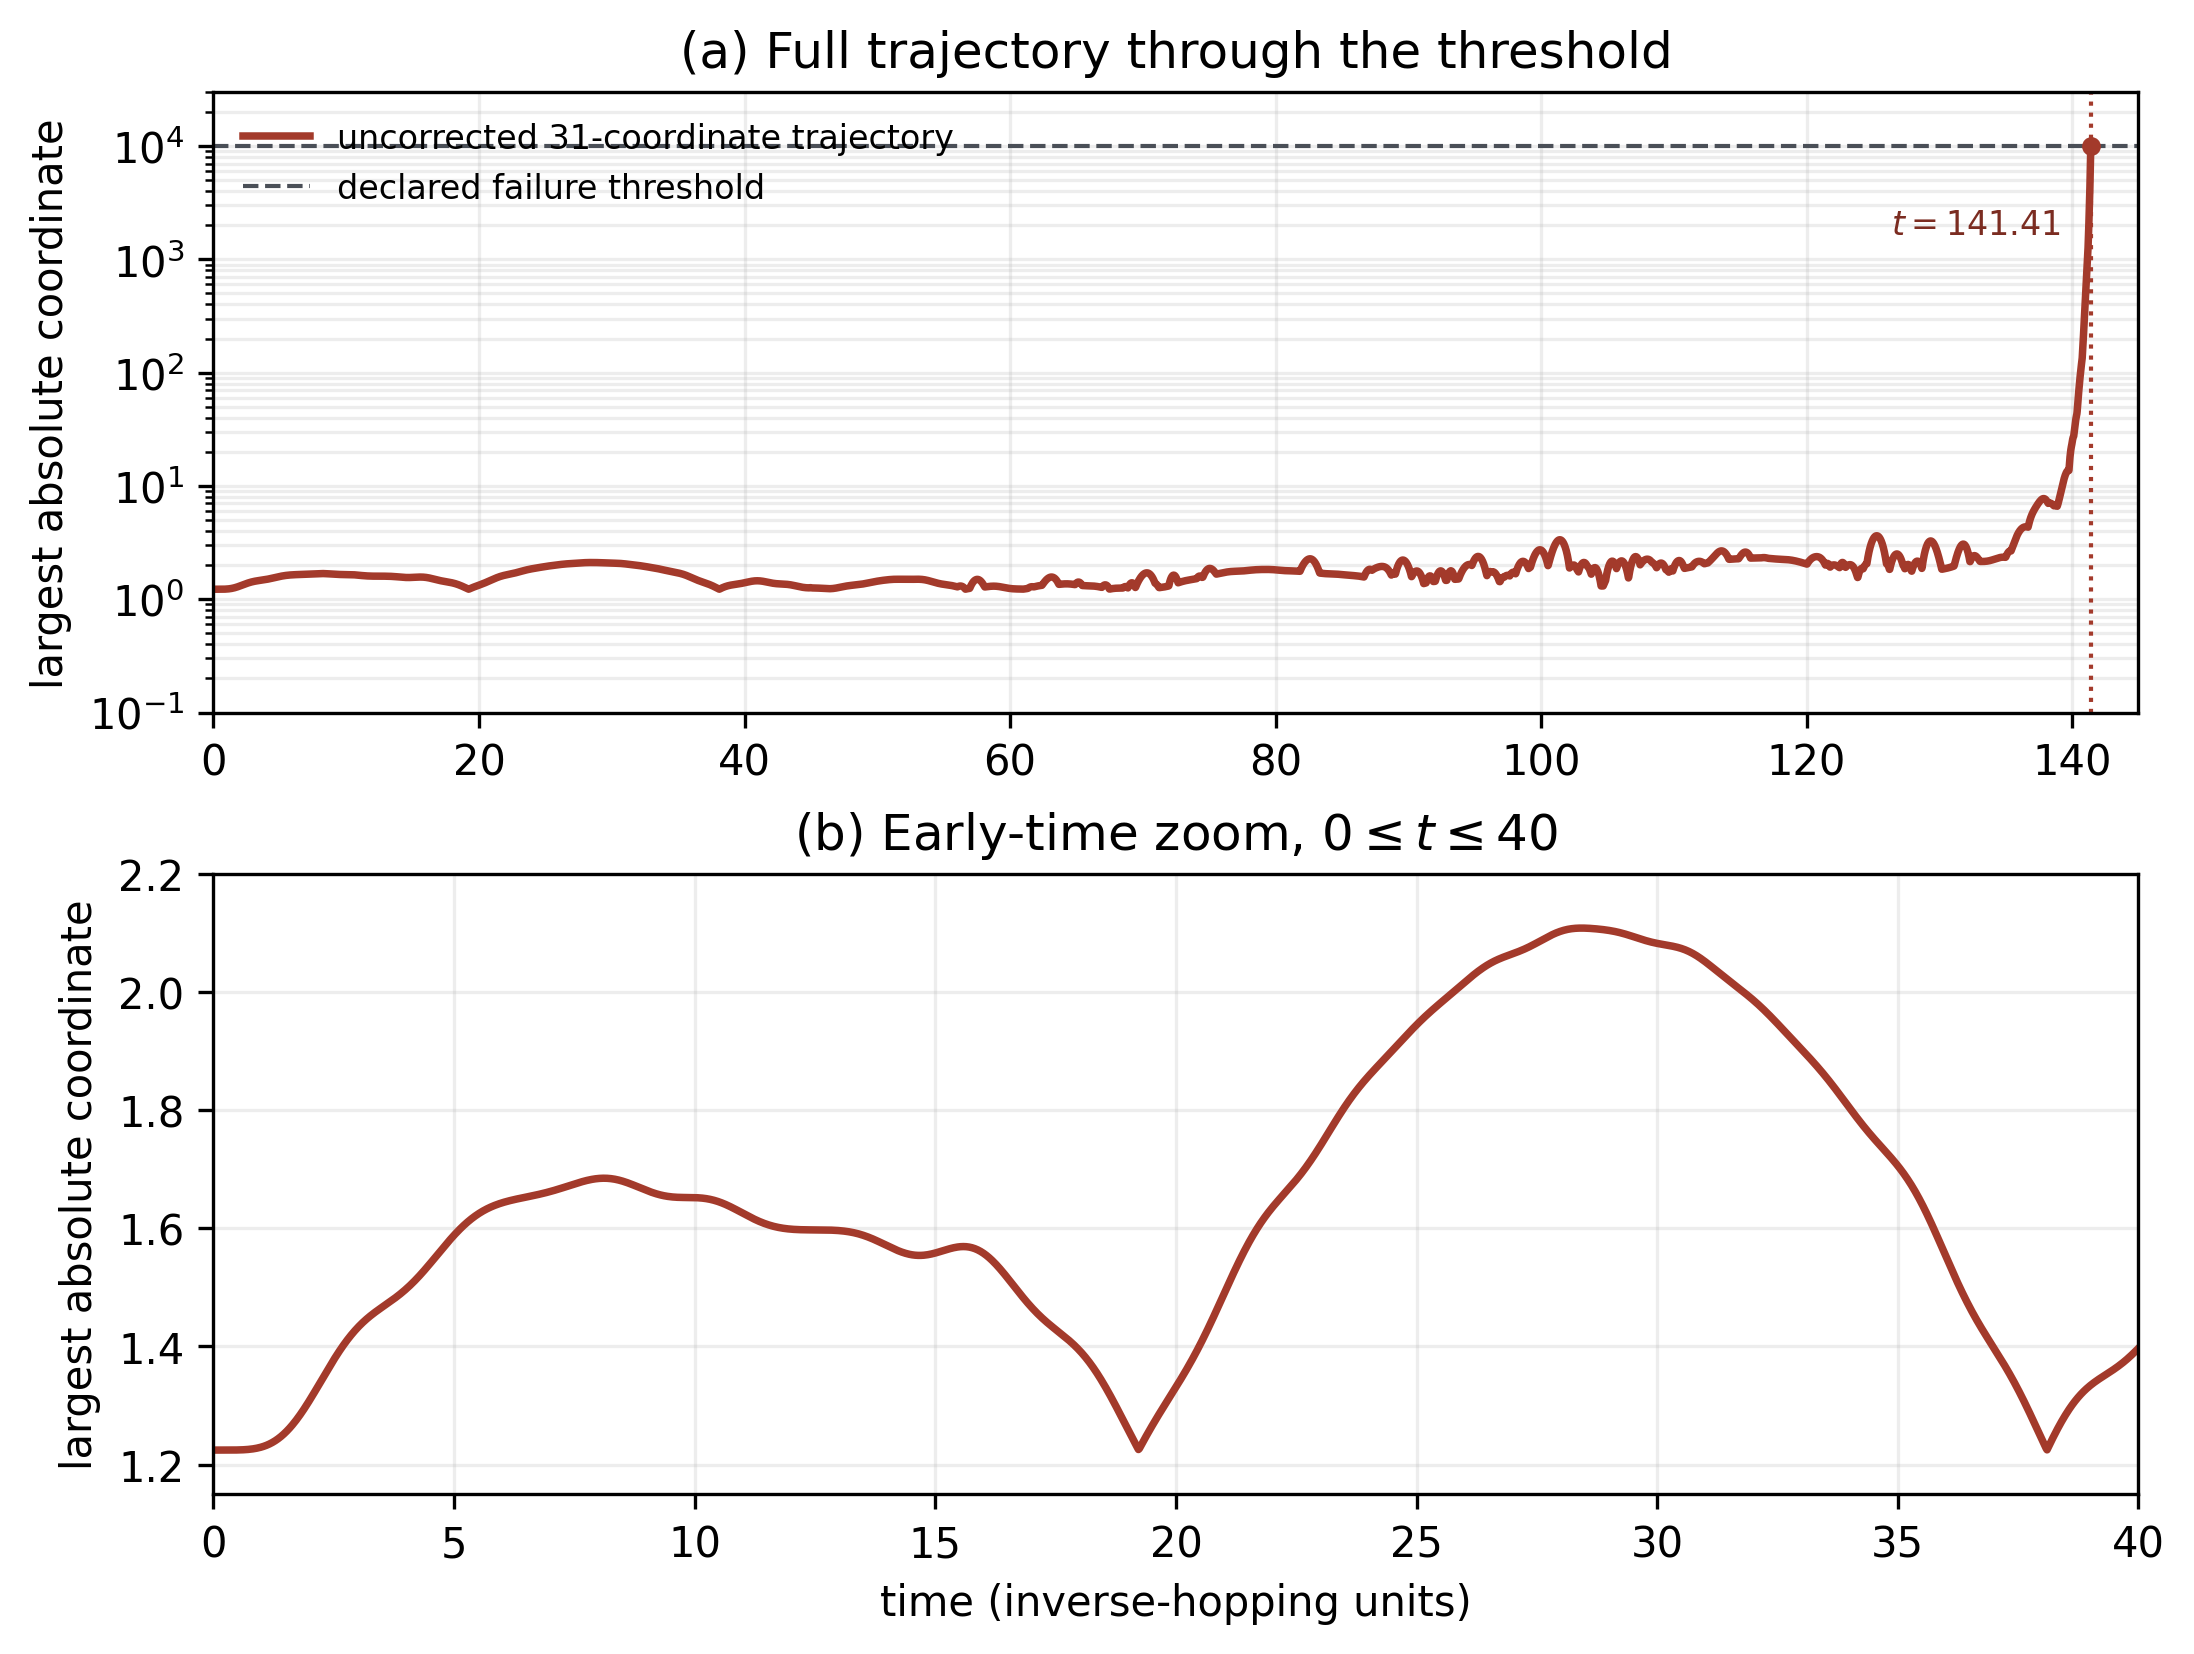
\includegraphics[width=\columnwidth]{advisor_project_overview_assets/paper_v/paper_v_divergence_reproduction_multiscale.pdf}
\caption{Uncorrected 31-coordinate trajectory.  Panel (a) shows the
logarithmic trajectory through $\norm{x}_\infty=10^4$; panel (b) resolves the
early oscillations on a linear vertical scale.}
\label{fig:divergence}
\end{figure}

Over $0\leq t\leq4\,t_{\rm hop}^{-1}$, the minimum joint-Gram eigenvalues
were
\begin{table}[H]
\centering
\small
\begin{tabular}{@{}lc@{}}
\toprule
trajectory & $\min_t\lambda_{\min}(\mathcal G)$\\
\midrule
exact cutoff-16 & $2.8524\times10^{-5}$\\
uncorrected archive & $-0.51727$\\
corrected archive & $2.0637\times10^{-5}$\\
\bottomrule
\end{tabular}
\caption{Joint-Gram physicality over the driven interval.}
\label{tab:joint-minima}
\end{table}

\begin{figure}[H]
\centering
\includegraphics[width=\columnwidth]{advisor_project_overview_assets/paper_v/paper_v_physicality_correction.pdf}
\caption{The uncorrected moment equations leave the joint Gram cone, while
the exact cutoff-16 and corrected trajectories retain nonnegative minimum
eigenvalues over the shown interval.}
\label{fig:physicality}
\end{figure}

The corrected $h=0.01\,t_{\rm hop}^{-1}$ trajectory contains $100{,}000$
RK4 steps through $t=1000$, hence $400{,}000$ constrained stage solves.  All
solves converged; the minimum joint-Gram margin was
$2.0637\times10^{-5}$ and the maximum post-pulse internal-energy change was
$5.03\times10^{-6}\,t_{\rm hop}$.

\subsection{Observable and block accuracy}

Figure~\ref{fig:observable-long} compares the archive observables with exact
cutoff-16 Hamiltonian propagation.  The raw component energies leave the
plotted physical range before their terminal blow-up.  Their cancellation in
the total internal energy demonstrates that a stable conserved sum does not
certify accurate component dynamics.

\begin{figure*}[t]
\centering
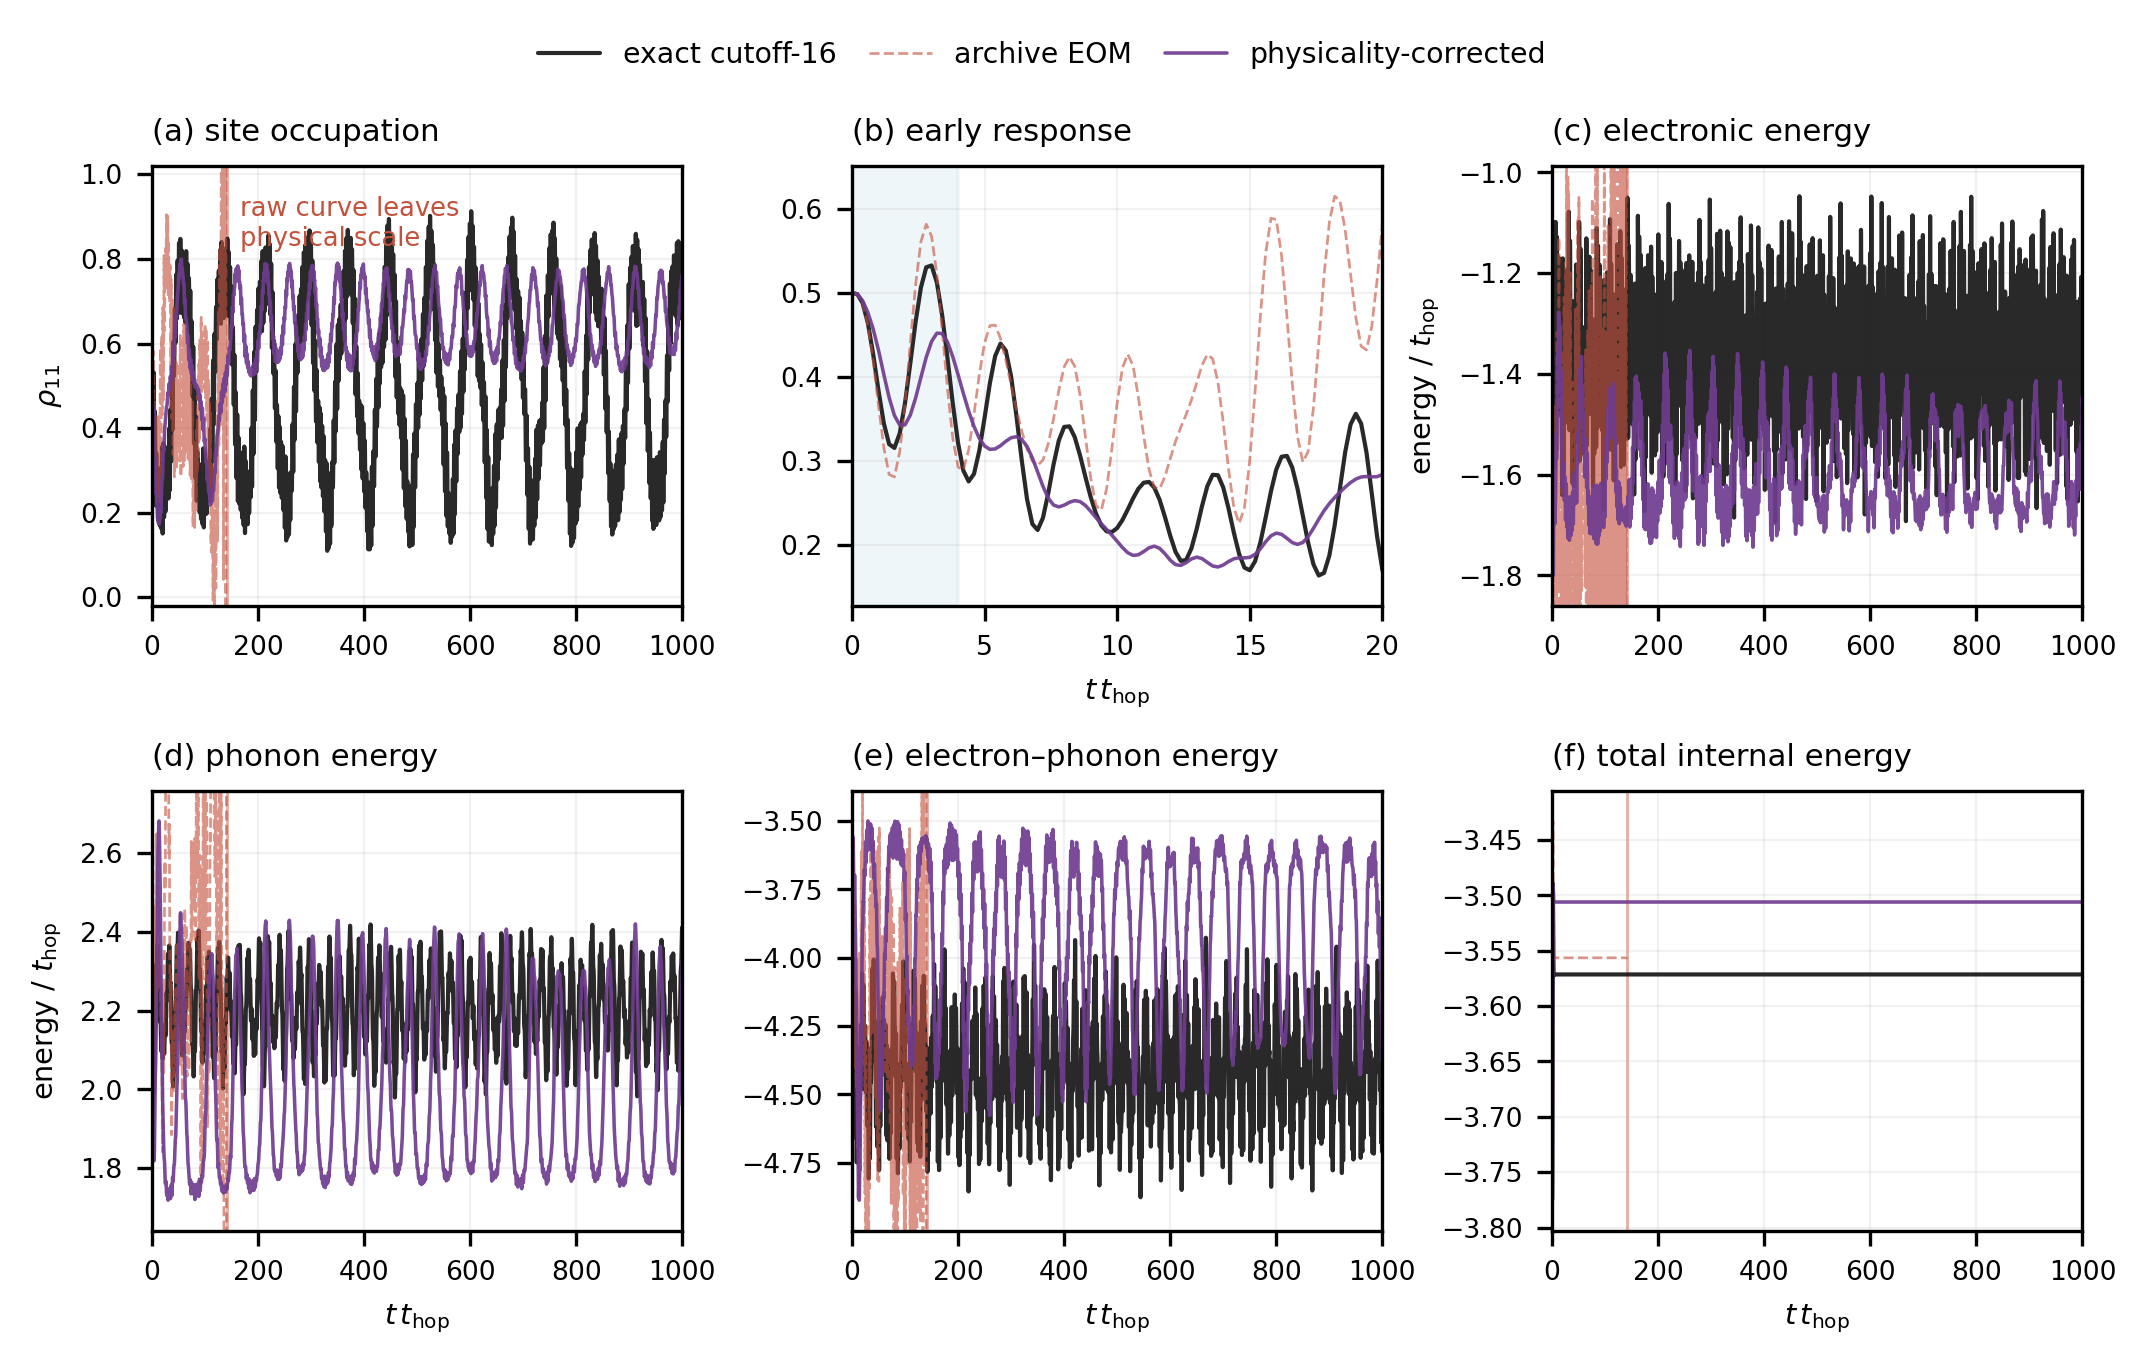
\includegraphics[width=0.98\textwidth]{advisor_project_overview_assets/paper_v/paper_v_archive_observable_trajectories.pdf}
\caption{Archive observables over the complete tested horizon.  Black is
exact cutoff-16 propagation, dashed red is the raw archive closure, and
purple is the Euclidean physicality-corrected closure.  Panel (b) expands the
first 20 time units; the vertical red line marks the raw amplitude-threshold
event.}
\label{fig:observable-long}
\end{figure*}

The matched $t\leq20$ metric ablation replaces the Euclidean objective by the
combined Frobenius norm of the lifted block corrections.  Relative to the
Euclidean correction, the Frobenius correction lowers the dynamic-normalized
errors in $\rho,B,N,$ and $C$, raises the $A$ error, and increases the
internal-energy RMS error from $0.06284$ to
$0.12788\,t_{\rm hop}$.  It therefore redistributes rather than uniformly
reduces the dynamical error.

\begin{figure*}[t]
\centering
\includegraphics[width=0.98\textwidth]{advisor_project_overview_assets/paper_v/paper_v_correction_metric_observables_t20.pdf}
\caption{Matched short-horizon observables.  Black is exact cutoff-16
propagation, dashed red is the raw archive closure, purple is the Euclidean
correction, and dash-dotted teal is the lifted-Frobenius correction.  Panel
(f) shows absolute internal-energy error; blue bands mark
$0\leq t\leq4\,t_{\rm hop}^{-1}$.}
\label{fig:observable-short}
\end{figure*}

For $Y\in\{\rho,B,N,A,C\}$ and trajectory $a$, define the
dynamic-normalized block error
\begin{equation}
e_Y^{(a)}(t;T)=
\frac{\norm{Y_a(t)-Y_{\rm ex}(t)}_{\rm F}}
{[T^{-1}\int_0^T\norm{Y_{\rm ex}(t)-Y_{\rm ex}(0)}_{\rm F}^2dt]^{1/2}}.
\label{eq:block-error}
\end{equation}
The raw errors grow without bound, whereas the corrected $T=1000$ time-RMS
errors remain finite: $(1.1951,1.2173,1.2761,1.2088,1.1733)$ in the order
$(\rho,B,N,A,C)$.  This is stabilization, not recovery of exact dynamics.

\begin{figure*}[t]
\centering
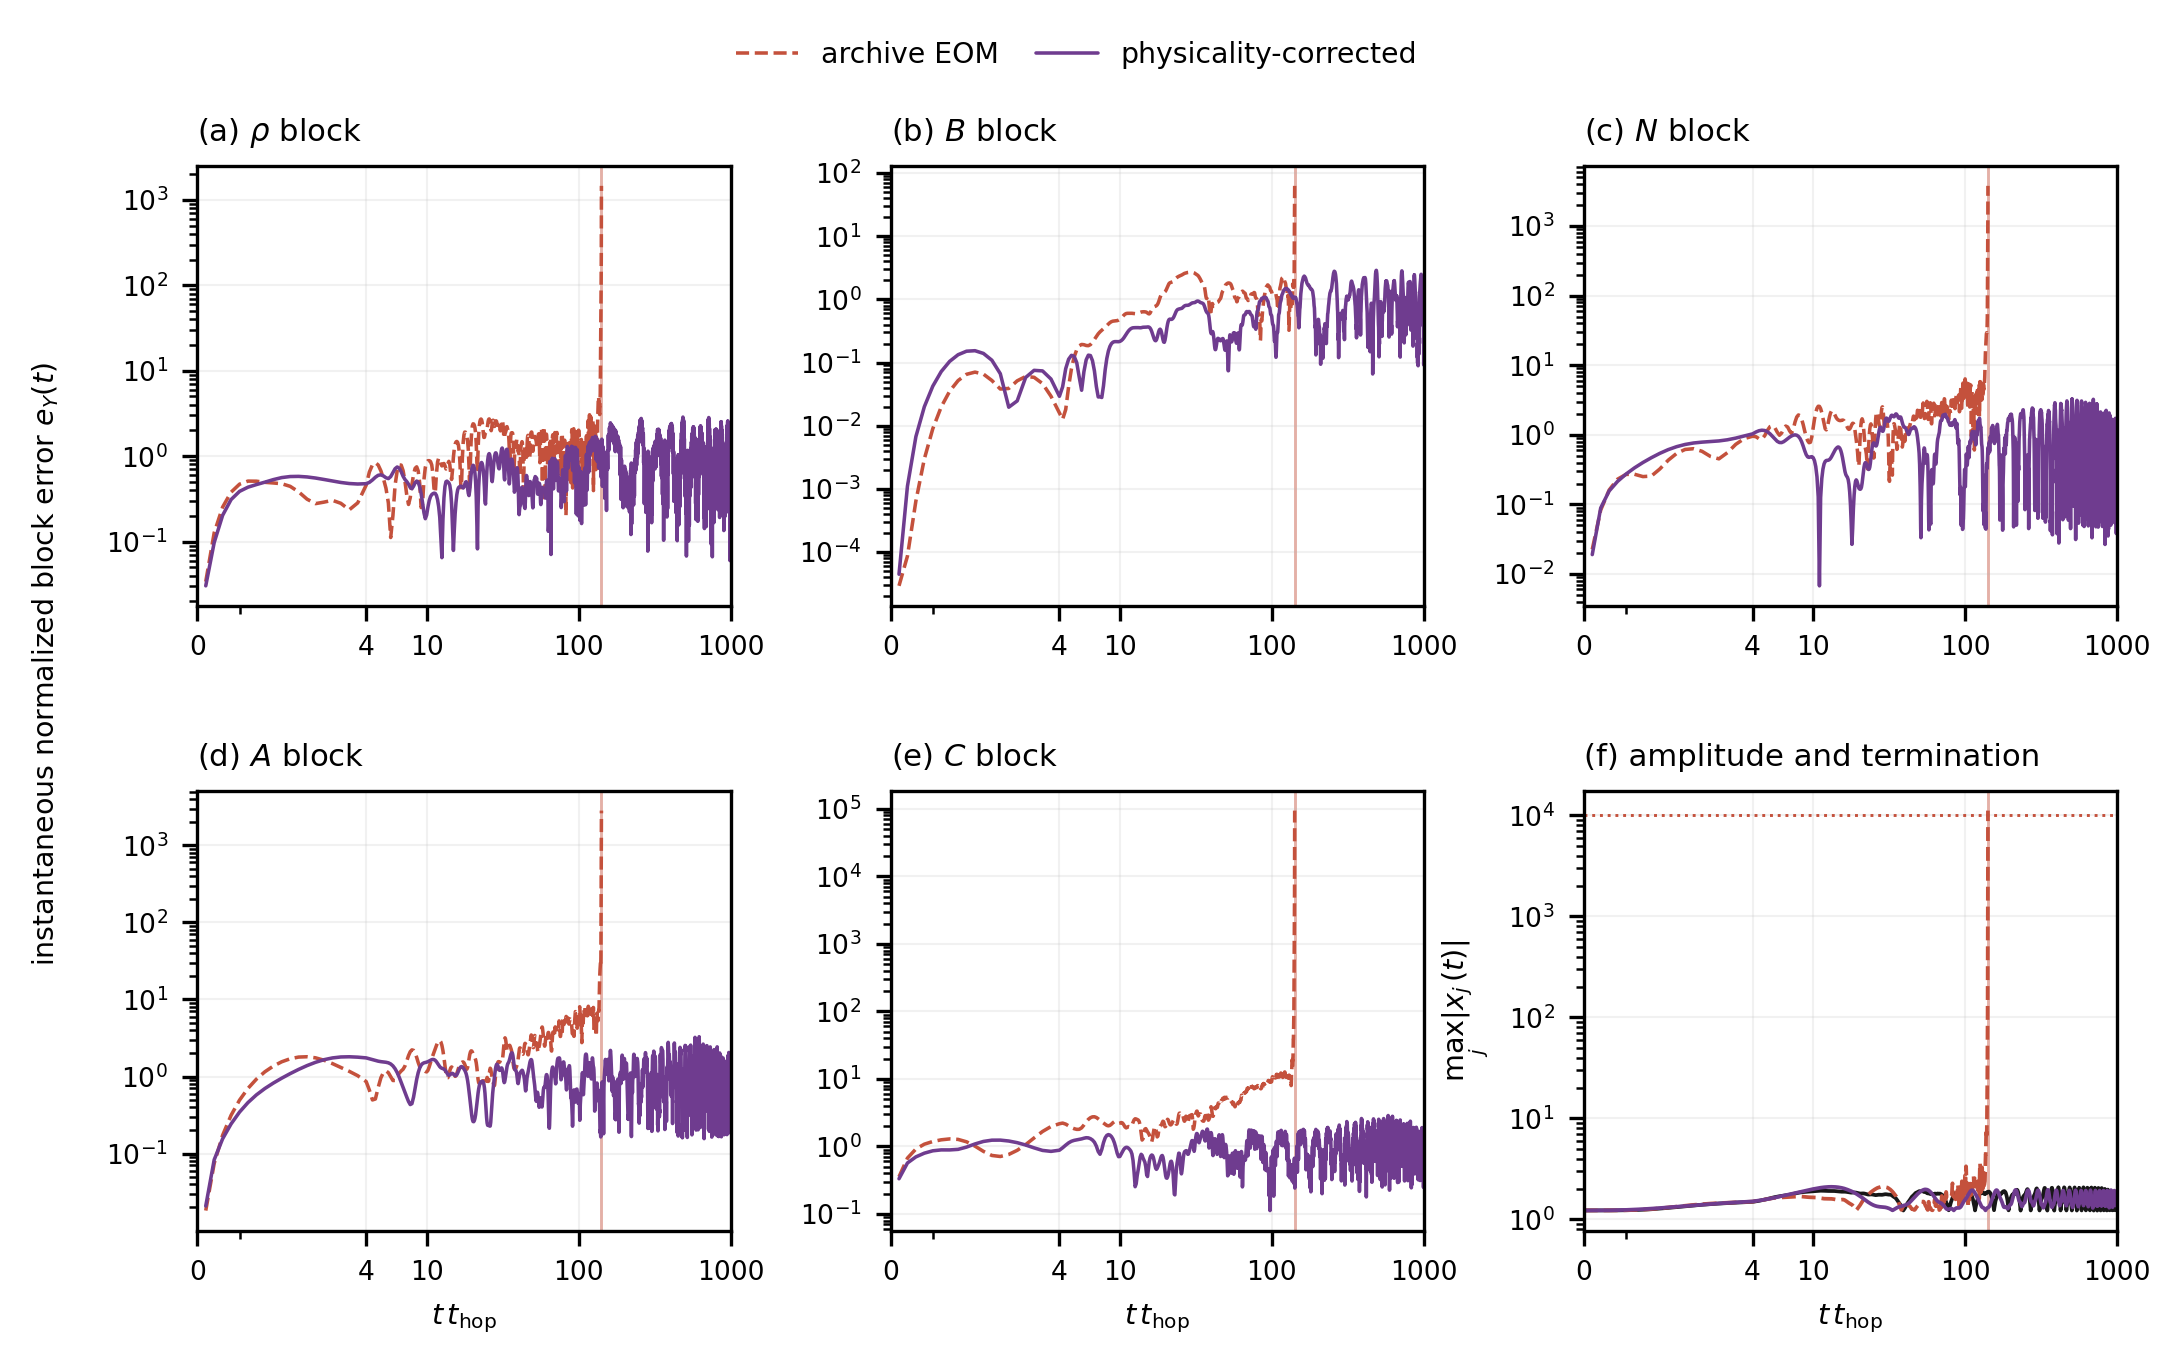
\includegraphics[width=0.98\textwidth]{advisor_project_overview_assets/paper_v/paper_v_block_error_trajectories.pdf}
\caption{Instantaneous dynamic-normalized errors from
Eq.~\eqref{eq:block-error}.  Panels (a)--(e) compare each retained moment
block with the exact cutoff-16 contraction; panel (f) shows the coordinate
amplitude and the $10^4$ declaration threshold.  The raw trajectory ends at
its divergence event and is not extrapolated.}
\label{fig:block-errors}
\end{figure*}

\subsection{Higher-order extensions move the terminal defect}

The exact-state audit localized the dominant local defect to the archive
$C$ velocity.  Retaining all symmetry-adapted moments through degree three
produces a 47-coordinate state and reduces the projected $C$-velocity RMS
defect to $1.01\times10^{-6}$; closing its new terminal equations with a zero
connected fourth cumulant nevertheless leaves a degree-three relative
derivative defect of $0.7302$.  Adding all 35 degree-four moments gives an
82-coordinate state and reduces the former degree-three defect to
$5.45\times10^{-6}$, while zero connected fifth cumulant leaves the new
degree-four terminal defect at $2.1276$.  Each extension repairs the previous
terminal block but transfers the dominant error to the newly highest order.

\section{Conclusion}

The archive moment equations fail first by leaving the joint
electron--phonon Gram cone, well before their terminal coordinate blow-up.
The minimum-Euclidean-norm differential correction preserves the tested
matrix and equality constraints and prevents divergence through the tested
$t=1000$ horizon.  Exact-reference observables and block errors remain
inaccurate, and direct order-by-order moment extension shifts rather than
eliminates the closure defect.

\clearpage
\appendix

\twocolumn[{
\section{Primitive calculation chain}
\label{app:primitive-chain}

\begin{minipage}{0.97\textwidth}
\footnotesize
Let $\langle O\rangle_0=\langle\Psi_0|O|\Psi_0\rangle$ denote an
expectation value in the exact cutoff-16 ground state.  The initial
contractions, their ordered real coordinates, one archive right-hand-side
evaluation, the joint-Gram test, and the corrected velocity form the single
composition
\begin{equation}
\begin{aligned}
|\Psi_0\rangle
&\xrightarrow{\ \langle\,\cdot\,\rangle_0\ }
\left\{
\begin{gathered}
\rho_{ij}(0)=\langle c_j^\dagger c_i\rangle_0,\quad
B_q(0)=\langle b_q\rangle_0,\quad
\delta b_q=b_q-B_q,\\
N_{qr}(0)=\langle\delta b_r^\dagger\delta b_q\rangle_0,\quad
A_{qr}(0)=\langle\delta b_q\delta b_r\rangle_0,\quad
C^q_{ij}(0)=\langle\delta b_q(c_j^\dagger c_i-\rho_{ij})\rangle_0
\end{gathered}
\right\}
=X(0),\\[2pt]
X
&\xrightarrow{\ \rho=\rho^\dagger,\ \Tr\rho=1,\ N=N^\dagger,\
A=A^{\mathsf T},\ \Tr C^0=\Tr C^1\ }
\left\{
\begin{gathered}
x_\rho=(n_-,\Re\rho_{01},\Im\rho_{01}),\\
x_B=(\Re B_0,\Im B_0,\Re B_1,\Im B_1),\\
x_N=(N_{00},N_{11},\Re N_{01},\Im N_{01}),\\
x_A=(\Re A_{00},\Im A_{00},\Re A_{11},\Im A_{11},\Re A_{01},\Im A_{01}),\\
x_C=(\Re s,\Im s,\Re d_0,\Im d_0,\Re u_0,\Im u_0,\Re v_0,\Im v_0,
\Re d_1,\Im d_1,\Re u_1,\Im u_1,\Re v_1,\Im v_1)
\end{gathered}
\right\},\\[-1pt]
&\hspace{2.0em}
n_-=\rho_{00}-\rho_{11},\quad s=\Tr C^0=\Tr C^1,\quad
d_q=C^q_{00}-C^q_{11},\quad u_q=C^q_{01},\quad v_q=C^q_{10},\\[-1pt]
&\hspace{2.0em}
x=x_\rho\oplus x_B\oplus x_N\oplus x_A\oplus x_C\in\R^{31},\\[2pt]
x(t)
&\xrightarrow{\ \text{reconstruct entries}\ }
\left\{
\begin{gathered}
\rho=\begin{pmatrix}(1+n_-)/2&\Re\rho_{01}+\ii\Im\rho_{01}\\
\Re\rho_{01}-\ii\Im\rho_{01}&(1-n_-)/2\end{pmatrix},
\qquad B_q=\Re B_q+\ii\Im B_q,\\
N=\begin{pmatrix}N_{00}&\Re N_{01}+\ii\Im N_{01}\\
\Re N_{01}-\ii\Im N_{01}&N_{11}\end{pmatrix},
\qquad A=\begin{pmatrix}A_{00}&A_{01}\\A_{01}&A_{11}\end{pmatrix},\\
C^q=\begin{pmatrix}(s+d_q)/2&u_q\\v_q&(s-d_q)/2\end{pmatrix}
\end{gathered}
\right\}=X(t),\\[2pt]
X(t)
&\xrightarrow{\ \text{archive Eqs.~\eqref{eq:dimer-eoms}--\eqref{eq:c-sources-b}}\ }
\dot X_0=(\dot\rho_0,\dot B_0,\dot N_0,\dot A_0,\dot C^0_0,\dot C^1_0),\\[2pt]
\dot X_0
&\xrightarrow{\ \text{extract the same entries in the same order}\ }
\left\{
\begin{gathered}
\dot x_{\rho,0}=((\dot\rho_0)_{00}-(\dot\rho_0)_{11},
\Re(\dot\rho_0)_{01},\Im(\dot\rho_0)_{01}),\\
\dot x_{B,0}=(\Re(\dot B_0)_0,\Im(\dot B_0)_0,\Re(\dot B_0)_1,\Im(\dot B_0)_1),\\
\dot x_{N,0}=((\dot N_0)_{00},(\dot N_0)_{11},
\Re(\dot N_0)_{01},\Im(\dot N_0)_{01}),\\
\dot x_{A,0}=(\Re(\dot A_0)_{00},\Im(\dot A_0)_{00},
\Re(\dot A_0)_{11},\Im(\dot A_0)_{11},
\Re(\dot A_0)_{01},\Im(\dot A_0)_{01}),\\
\dot x_{C,0}=(\Re\dot s_0,\Im\dot s_0,
\Re\dot d_{0,0},\Im\dot d_{0,0},\Re\dot u_{0,0},\Im\dot u_{0,0},
\Re\dot v_{0,0},\Im\dot v_{0,0},\\[-2pt]
\hspace{7.0em}\Re\dot d_{1,0},\Im\dot d_{1,0},
\Re\dot u_{1,0},\Im\dot u_{1,0},\Re\dot v_{1,0},\Im\dot v_{1,0})
\end{gathered}
\right\},\\[-1pt]
&\hspace{2.0em}
\dot s_0=\Tr\dot C^0_0=\Tr\dot C^1_0,\quad
\dot d_{q,0}=(\dot C^q_0)_{00}-(\dot C^q_0)_{11},\quad
\dot u_{q,0}=(\dot C^q_0)_{01},\quad \dot v_{q,0}=(\dot C^q_0)_{10},\\[-1pt]
&\hspace{2.0em}
\dot x_0=\dot x_{\rho,0}\oplus\dot x_{B,0}\oplus\dot x_{N,0}
\oplus\dot x_{A,0}\oplus\dot x_{C,0}=f(t,x),\\[2pt]
X(t)
&\xrightarrow{\ r_a=\Tr(\rho\sigma_a),\ \delta\sigma_a=\sigma_a-r_a\I_2\ }
Y=(\delta b_0,\delta b_1,\delta b_0^\dagger,\delta b_1^\dagger,
\delta\sigma_x,\delta\sigma_y,\delta\sigma_z),\\[-1pt]
Y
&\xrightarrow{\ \mathcal G_{ab}=\langle Y_a^\dagger Y_b\rangle\ }
\mathcal G=
\begin{pmatrix}
N^{\mathsf T}&A^*&c^*\\
A&\I_2+N&c\\
c^{\mathsf T}&c^\dagger&E
\end{pmatrix},\qquad
c_{qa}=\Tr(C^q\sigma_a),\quad
E_{ab}=\Tr(\rho\sigma_a\sigma_b)-r_ar_b,\\[-1pt]
&\hspace{2.0em}
z^\dagger\mathcal Gz=
\left\langle\left(\sum_a z_aY_a\right)^\dagger
\left(\sum_b z_bY_b\right)\right\rangle\geq0,\\[2pt]
\dot X_0
&\longmapsto
\dot r_{a,0}=\Tr(\dot\rho_0\sigma_a),\quad
\dot c_{qa,0}=\Tr(\dot C^q_0\sigma_a),\quad
(\dot E_0)_{ab}=\Tr(\dot\rho_0\sigma_a\sigma_b)-\dot r_{a,0}r_b-r_a\dot r_{b,0},\\[-1pt]
&\hspace{2.0em}
\dot{\mathcal G}_0=
\begin{pmatrix}
\dot N_0^{\mathsf T}&\dot A_0^*&\dot c_0^*\\
\dot A_0&\dot N_0&\dot c_0\\
\dot c_0^{\mathsf T}&\dot c_0^\dagger&\dot E_0
\end{pmatrix},\\[2pt]
(x,\dot x_0,\mathcal G,\dot{\mathcal G}_0)
&\xrightarrow{\ \substack{w\in\R^{31}\ \text{lifted in the same ordered basis}\\
\text{and constrained by Eq.~\eqref{eq:correction-sdp}}}\ }
w^*=\arg\min_w\tfrac12\norm w_2^2,
\qquad
\dot x_{\rm c}=\dot x_0+w^*,\\[-1pt]
\dot x_{\rm c}
&\xrightarrow{\ \text{one corrected Runge--Kutta stage}\ }
x\ \text{at the next stage, where the entire chain is evaluated again.}
\end{aligned}
\label{eq:primitive-calculation-chain}
\end{equation}
The bracket $\langle Y_a^\dagger Y_b\rangle$ is the same quantum expectation
operation used in the first line, now applied to every pair of centered
directions.  These pairwise expectations assemble the representability test
$\mathcal G$.  The correction begins in the penultimate line: $w$ changes the
velocity, and the following appendix displays its matrix lift entry by entry.
\end{minipage}
\vspace{0.6em}
}]

\clearpage
\raggedbottom

\section{Block-affine reconstruction and correction lift}
\label{app:block-affine}

The coordinates in Eq.~\eqref{eq:coordinate-blocks} reconstruct the retained
matrices as
\begin{equation}
\begin{gathered}
\rho=\begin{pmatrix}
(1+n_-)/2&\Re\rho_{01}+\ii\Im\rho_{01}\\
\Re\rho_{01}-\ii\Im\rho_{01}&(1-n_-)/2
\end{pmatrix},\\
N=\begin{pmatrix}N_{00}&\Re N_{01}+\ii\Im N_{01}\\
\Re N_{01}-\ii\Im N_{01}&N_{11}\end{pmatrix},\\
A=\begin{pmatrix}A_{00}&A_{01}\\A_{01}&A_{11}\end{pmatrix},\qquad
B_q=\Re B_q+\ii\Im B_q,\\
C^q=\begin{pmatrix}(s+d_q)/2&u_q\\v_q&(s-d_q)/2\end{pmatrix}.
\end{gathered}
\label{eq:reconstruction}
\end{equation}
Replacing the independent coordinates in Eq.~\eqref{eq:reconstruction} by
the corresponding entries of $w=(w_0,\ldots,w_{30})$ gives the velocity
lift.  Explicitly,
\begin{equation}
\begin{gathered}
\Delta\dot\rho=\begin{pmatrix}w_0/2&w_1+\ii w_2\\w_1-\ii w_2&-w_0/2\end{pmatrix},\\
\Delta\dot B=\binom{w_3+\ii w_4}{w_5+\ii w_6},\\
\Delta\dot N=\begin{pmatrix}w_7&w_9+\ii w_{10}\\w_9-\ii w_{10}&w_8\end{pmatrix},\\
\Delta\dot A=\begin{pmatrix}
w_{11}+\ii w_{12}&w_{15}+\ii w_{16}\\
w_{15}+\ii w_{16}&w_{13}+\ii w_{14}
\end{pmatrix}.
\end{gathered}
\label{eq:lift-rho-bna}
\end{equation}
For $q=0,1$, let $(j_q,k_q)=(19,21)$ and $(25,27)$, respectively.  Then
\begin{equation}
\begin{gathered}
\widehat s=w_{17}+\ii w_{18},\qquad
\widehat d_q=w_{j_q}+\ii w_{j_q+1},\\
\widehat u_q=w_{k_q}+\ii w_{k_q+1},\qquad
\widehat v_q=w_{k_q+2}+\ii w_{k_q+3},\\
\Delta\dot C^q=
\begin{pmatrix}
\frac{\widehat s+\widehat d_q}{2}&\widehat u_q\\
\widehat v_q&\frac{\widehat s-\widehat d_q}{2}
\end{pmatrix}.
\end{gathered}
\label{eq:lift-c}
\end{equation}
The lifted joint-Gram velocity follows without new degrees of freedom:
\begin{equation}
\begin{aligned}
\Delta\dot\MB&=\begin{pmatrix}
\Delta\dot N^{\mathsf T}&\Delta\dot A^*\\
\Delta\dot A&\Delta\dot N
\end{pmatrix},\\
(\Delta\dot E)_{ab}&=\Tr(\Delta\dot\rho\,\sigma_a\sigma_b)
-\Delta r_ar_b-r_a\Delta r_b,\\
\Delta\dot Z&=\binom{\Delta c^*}{\Delta c},\\
\Delta\dot{\mathcal G}=\begin{pmatrix}
\Delta\dot\MB&\Delta\dot Z\\
\Delta\dot Z^\dagger&\Delta\dot E
\end{pmatrix},
\end{aligned}
\label{eq:joint-lift}
\end{equation}
where $\Delta r_a=\Tr(\Delta\dot\rho\,\sigma_a)$ and
$\Delta c_{qa}=\Tr(\Delta\dot C^q\sigma_a)$.

\section{Euclidean minimum by equality elimination and eigenvector cuts}
\label{app:minimum-solution}

Collect the real and imaginary trace equations and the energy-neutrality row
of Eq.~\eqref{eq:correction-sdp} into
$L_{\rm eq}w=d_{\rm eq}$.  An SVD gives
\begin{equation}
\begin{gathered}
w=w_{\rm p}+Zy,\qquad w_{\rm p}=L_{\rm eq}^{+}d_{\rm eq},\\
L_{\rm eq}Z=0,\qquad Z^{\mathsf T}Z=\I.
\end{gathered}
\label{eq:nullspace}
\end{equation}
Because $w_{\rm p}$ is orthogonal to the null space,
$\norm{w}_2^2=\norm{w_{\rm p}}_2^2+\norm y_2^2$.  Each barrier matrix is
affine in $y$:
\begin{equation}
\begin{gathered}
B_\ell(y)=M_{0,\ell}+\Delta M_\ell(w_{\rm p}+Zy),\\
\ell\in\{\rho,\I_2-\rho,\mathcal G\}.
\end{gathered}
\label{eq:affine-barrier}
\end{equation}
If $B_\ell(y^{(k)})v=\lambda v$ with $\lambda<0$ and $v^\dagger v=1$, define
$[a_\ell(v)]_j=v^\dagger\Delta M_\ell(e_j)v$ and
$n=Z^{\mathsf T}a_\ell(v)$.  Affinity gives the exact half-space cut
\begin{equation}
n^{\mathsf T}y\geq n^{\mathsf T}y^{(k)}-\lambda.
\label{eq:eigenvector-cut}
\end{equation}
After the currently exposed negative modes, SLSQP solves
\begin{equation}
\min_y\tfrac12y^{\mathsf T}y
\quad\text{subject to}\quad n_i^{\mathsf T}y\geq c_i.
\label{eq:cutting-plane-qp}
\end{equation}
The complete barrier matrices are then diagonalized, newly violated
eigenvector cuts are appended, and the quadratic program is repeated until
all three matrices satisfy Eq.~\eqref{eq:correction-sdp}.  The resulting
$w^*=w_{\rm p}+Zy^*$ is therefore the Euclidean-minimum feasible correction
in the chosen 31-coordinate scaling.

\begin{thebibliography}{9}
\small
\raggedright

\bibitem{riva2026}
G.~Riva, J.~Simoni, and Y.~Ping,
``Open-quantum-system theory of non-Markovian electron--phonon dynamics,''
arXiv:2606.22233 (2026).

\bibitem{hornJohnson2012}
R.~A. Horn and C.~R. Johnson,
\emph{Matrix Analysis}, 2nd ed. (Cambridge University Press, Cambridge,
2012), doi:10.1017/CBO9781139020411.

\bibitem{kato1966}
T.~Kato, \emph{Perturbation Theory for Linear Operators}
(Springer, Berlin, 1966), doi:10.1007/978-3-662-12678-3.

\bibitem{ong2025}
P.~Ong, Y.~Xu, R.~M.~Bena, F.~Jabbari, and A.~D.~Ames,
``Matrix control barrier functions,'' arXiv:2508.11795v2 (2025),
doi:10.48550/arXiv.2508.11795.

\bibitem{vandenbergheBoyd1996}
L.~Vandenberghe and S.~Boyd, ``Semidefinite programming,''
SIAM Rev. \textbf{38}, 49--95 (1996), doi:10.1137/1038003.

\end{thebibliography}

\end{document}
